\chapterp{3p}{Online band-pass filters}\label{sec:BPF}

This section explores the current state-of-the-art method in online ripple detection (\cref{sec:offline} discussed \emph{offline} ripple detection), namely the online band-pass filter. \Cref{sec:eval} showed how we form detections 
% todo: mention adaptive threshold

\clearpage
\begin{figure}
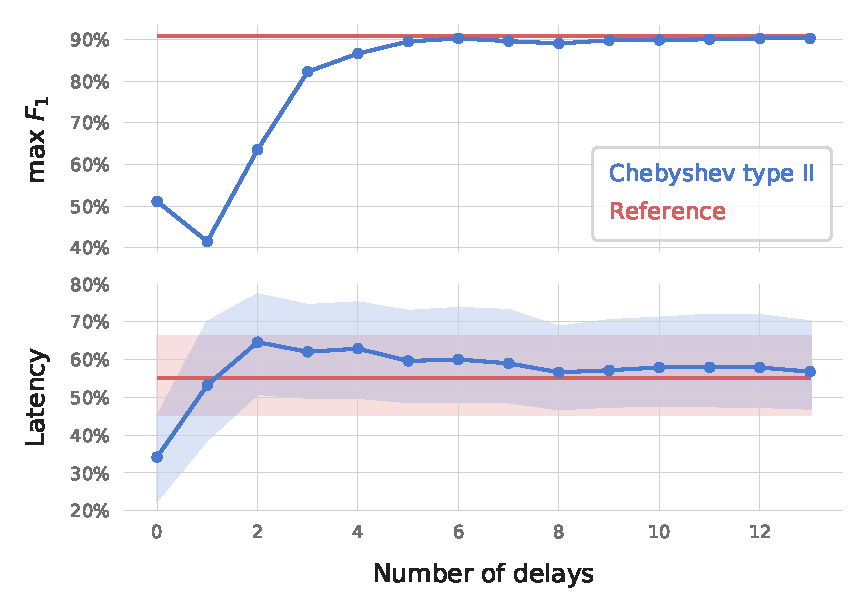
\includegraphics{figures/searcharray-cheby2}
\captionn[, ]{Performance of Chebyshev type 2 IIR-filters}{for different filter orders. The minimum stop-band attenuation was set to 40 dB.}
\end{figure}

\begin{figure}
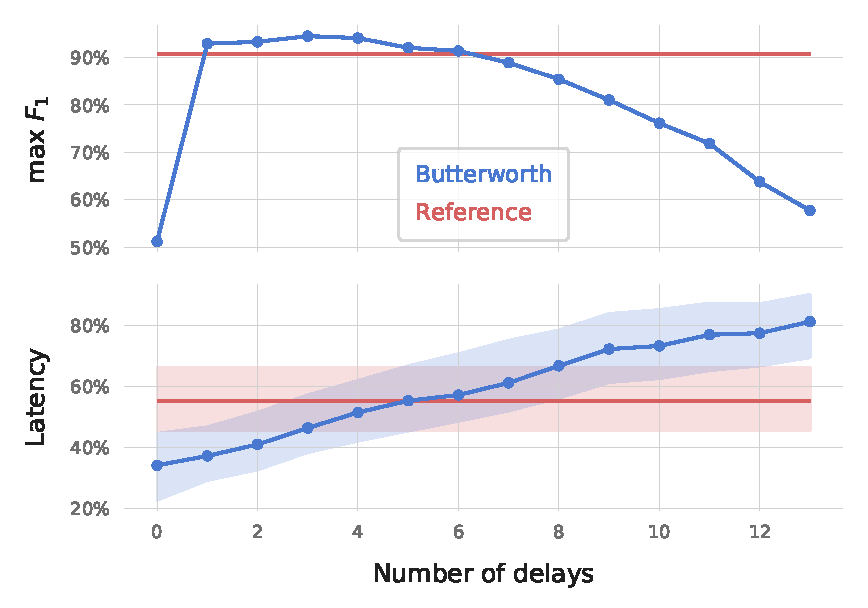
\includegraphics{figures/searcharray-butter}
\captionn[, ]{Performance of Butterworth IIR-filters}{for different filter orders.}
\end{figure}
